\documentclass[aps,prb,10pt,twocolumn,groupedaddress]{revtex4-1}
%\setlength\topmargin{4.6mm}
%\documentclass{[prl,twocolumn]{revtex4-1}
%\usepackage[ansinew]{inputenc}
%\usepackage[latin1]{inputenc}% PROPER ENCODINGS
%\usepackage[T1]{fontenc}%      FOR FINNISH TEXT
%\usepackage[finnish]{babel}% 
%\usepackage[official]{eurosym}

%\usepackage{subfig}
\usepackage{caption}
\usepackage{subcaption}
\usepackage{graphicx}
\usepackage{epsfig}
\usepackage{epstopdf}
\usepackage{amsmath}
\usepackage{blkarray}
\usepackage{multirow}
\usepackage{mathtools}
\usepackage[font=small,labelfont=bf]{caption}
\usepackage{listings}

%\usepackage{subfig}
%\usepackage[footnotesize]{caption}
%\pagestyle{empty}
%\setlength{\textwidth}{140mm}
%\setlength{\textheight}{240mm}
%\setlength{\parindent}{0mm}
%\setlength{\parskip}{3mm plus0.5mm minus0.5mm}
\bibliographystyle{apsrev4-1}
%%%%%%%%%%%%%%%%%%%%%%%%%%%%%%%%%%
\begin{document}

\title{Automatic Detection of Blood Vessels From Retinal Images Using Convolutional Neural Network }
\date{\today}
\author{Ville Virkkala, Jarno Leppänen}

\begin{abstract}
Main causes of blindness, such as diabetes and hypertension, are related	to morphological changes of the blood vessels. Thus automatic segmentation of blood vessels from retinal images could greatly improve to make the correct diagnosis in
optometric studies. In this work a convolutional neural network is developed to automatically segment blood vessels from retinal images. The developed method produces an accuracy of 85\% for the test set. The performance of developed method is also compared against other similar mehthods and against random forest classifier. 
\end{abstract}

\maketitle

\section{Introduction}

Several studies have used neural networks in automatic blood vessel detection from retinal images. These methods can be roughly divided into two groups: patch based segmentation of blood vessels\cite{tan} and methods based on fully convolutional neural networks\cite{long,hu}. In patch based image segmentation the image is traversed through pixel by pixel. For each pixel a patch of fixed size, centered at the pixel, is taken from the image and fed to neural network that classifies the pixel into certain class. In Ref. \cite{tan}, for each pixel three patches of different sizes from the green channel of image were taken and scaled into same size and used as a three channel input to convolutional neural network. In Ref. \cite{tan} the reported accuracy was in most cases clearly better than 90\%. 
The advantages of patch based method are their simplicity and ease of training. However, their main disadvantage is the high computational load when doing inference, because for each pixel separate patch is taken that is fed to neural network. Fully convolutional neural networks\cite{long} are the current state of the art method in image segmentation. The huge advantage of fully convolutional neural network is the huge speed up compared to patch based methods, because the whole image is fed only once as whole to the neural network. In addition there is more contextual information available in fully convolutional neural networks because the whole image is processed at once instead of using smaller patches. In Ref. \cite{hu} a modified version of the fully convolutional network in Ref. \cite{long} was used. In Ref. \cite{hu} the downsampling of the image was done using the same VGG-16 network as in \cite{long} however the output of each convolution stage was directly upsampled into original size and a binary cross entropy loss was then connected into each upsampled image. The final loss that was optimized is then the sum of the losses connected to each upsampled image. In Ref. \cite{hu} the reported accuracy was in all cases better than 95\% while the method was much faster, single image segmentation time around 11seconds, than the method of Ref. \cite{tan}, single image segmentation time around 2000 seconds.  

In this work a patch based semantic segmentation method based on convolutional neural networks, resembling that of Ref. \cite{tan},  is developed to detect blood vessels from retinal images. The performance of the developed method is validated against several test images. In addition performance of the developed method is compared to random forest classifier implemented in scikit-learn python library \cite{scikit-learn}.
The paper is organized as follows. The used data-set and the computational
methods are described in detail in sections \ref{sec:used_data_set} and \ref{sec:computational_methods}. In Sec. \ref{sec:results} training metrics and performance of the developed method in inference when applied on test images are given.
Sec. \ref{sec:conclusions} is a summary of the results and the differences between the two classifiers are discussed.

\section{Used data-set}
\label{sec:used_data_set}
The used data set in this work is the publicly available DRIVE data set \cite{staal} available in \cite{driveurl}. The data set consist of 40 images of size 565x584 and the corresponding ground truth annotations of blood vessels. The images were obtained from diabetic subjects as a part of diabetic retinopathy screening program in The Netherlands.

The data set was divided into training, validation and test sets containing 28, 6 and 6 images respectively. The images are three channel RGB images, but only the green channel is used in classification, because of the high contrast between blood vessels and background in green channel\cite{green_contrast}. In classification of pixels patches of size 33x33 centered at the pixel were used. From each image 2000 patches for both pixels corresponding to blood vessels and background pixels were randomly sampled resulting in total of 112000 samples for training set, 24000 samples for validation set and 24000 samples for test set respectively. Examples of retinal image that is classified and the corresponding ground truth image are shown in figures \ref{fig:example_images}a and \ref{fig:example_images}b respectively. Examples of patches that corresponds to pixels that are labeled as blood vessels and background are shown in figures \ref{fig:example_patches}a-\ref{fig:example_patches}c and \ref{fig:example_patches}d-\ref{fig:example_patches}f respectively.
\begin{figure*}[!t]
	\centering
	\begin{subfigure}[]{0.4\textwidth}
		\centering
		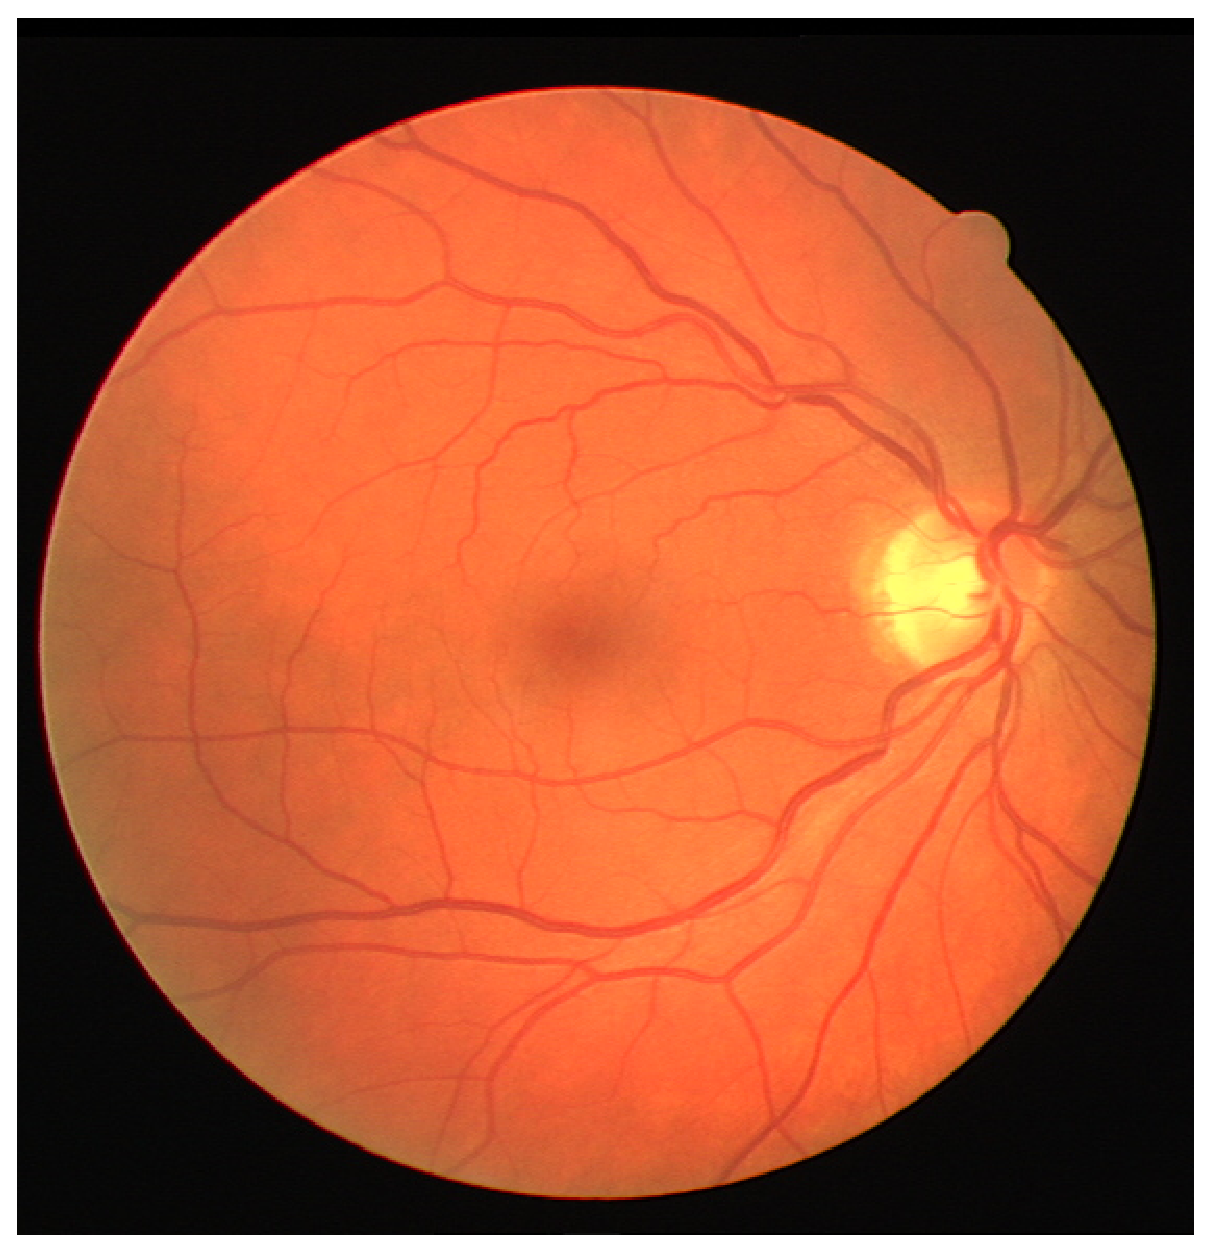
\includegraphics[width=\textwidth]{images/02_training.eps}
		\caption{}
	\end{subfigure}
	\hspace{1cm}
	\centering
	\begin{subfigure}[]{0.4\textwidth}
		\centering
		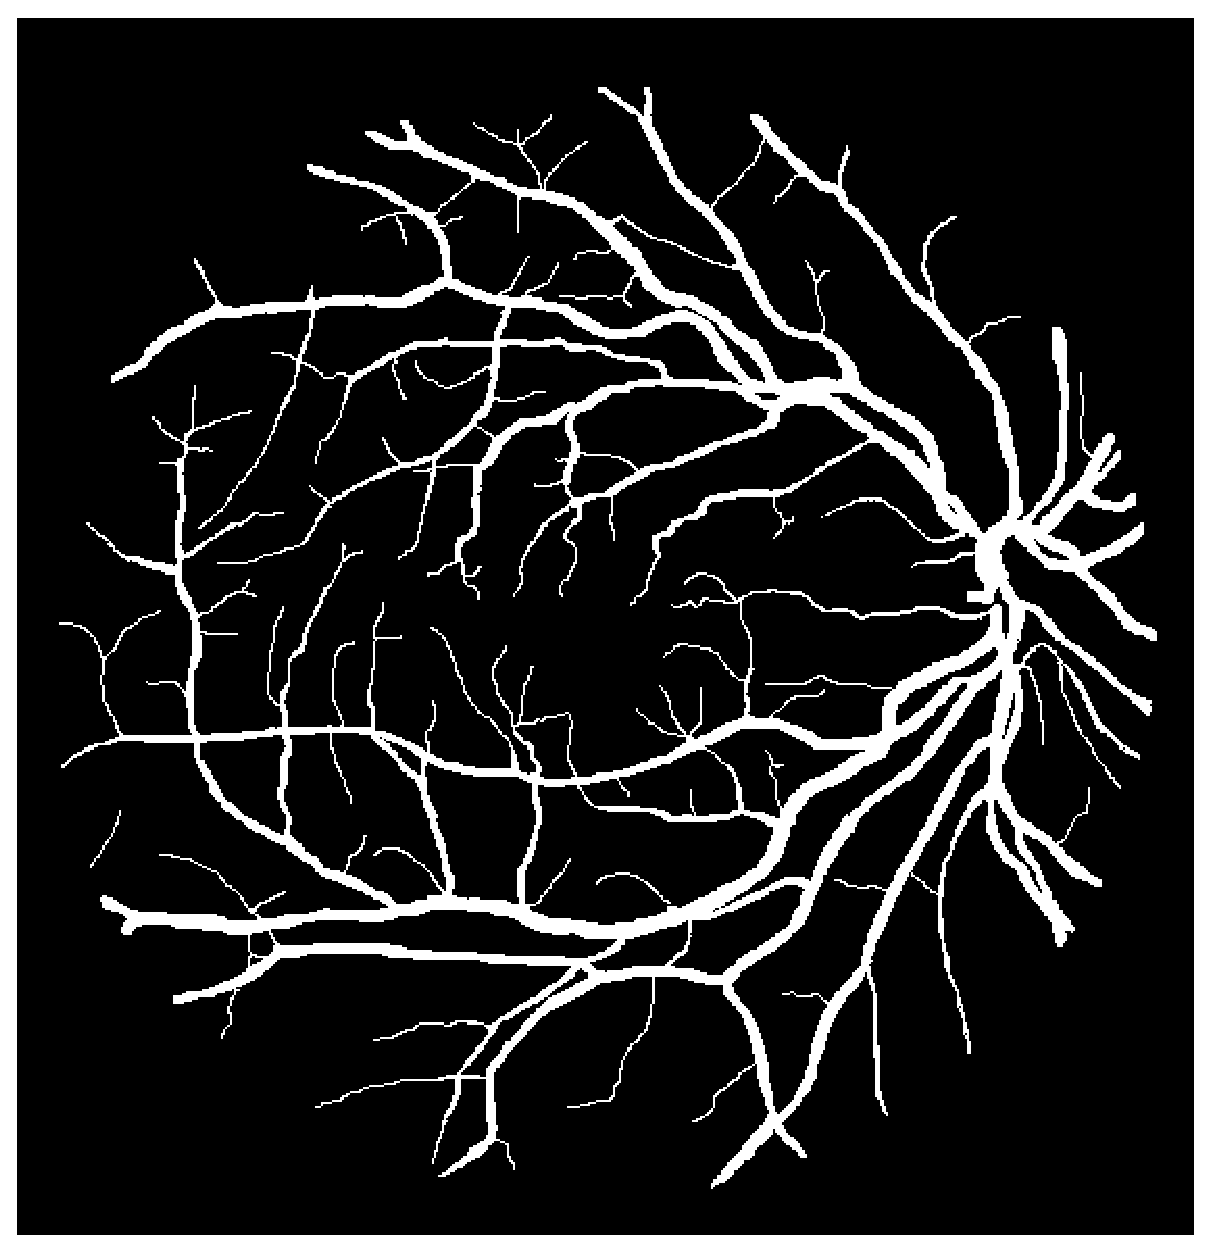
\includegraphics[width=\textwidth]{images/02_manual1.eps}
		\caption{}
	\end{subfigure}\\
	\caption{Example of retinal image used in training (a) and the corresponding ground truth annotation of blood vessels (b).}
	\label{fig:example_images}
\end{figure*}

\section{Computational methods}
\label{sec:computational_methods}
The developed neural network in this work is implemented using the Python programming language and the PyTorch\cite{pytorch} open-source machine learning library for Python. The reference, random-forest classifier, method is implemented using the Scikit-learn machine learning library\cite{scikit-learn}. The source code for most relevant parts of the algorithm are given in Appendix \ref{appendix:a}
\begin{figure*}[!t]
	\centering
	\begin{subfigure}[]{0.22\textwidth}
		\centering
		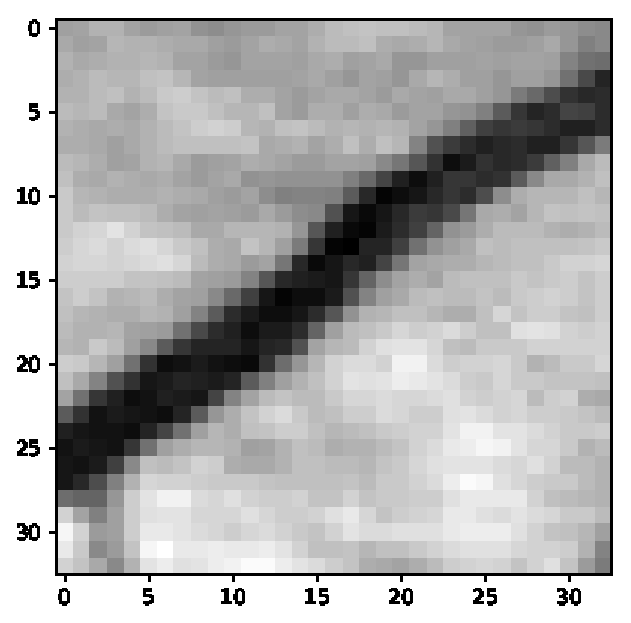
\includegraphics[width=\textwidth]{images/positive1.eps}
		\caption{}
	\end{subfigure}
	\hspace{1.55cm}
	\centering
	\begin{subfigure}[]{0.22\textwidth}
		\centering
		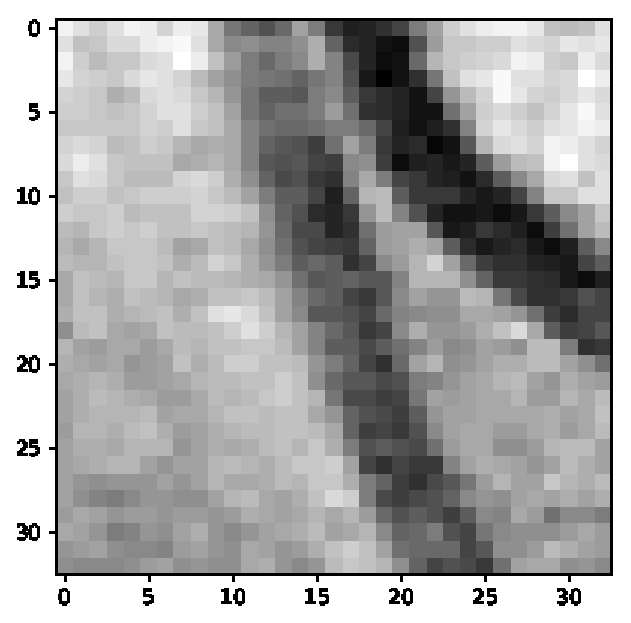
\includegraphics[width=\textwidth]{images/positive2.eps}
		\caption{}
	\end{subfigure}
	\hspace{1.55cm}
	\centering
	\begin{subfigure}[]{0.22\textwidth}
		\centering
		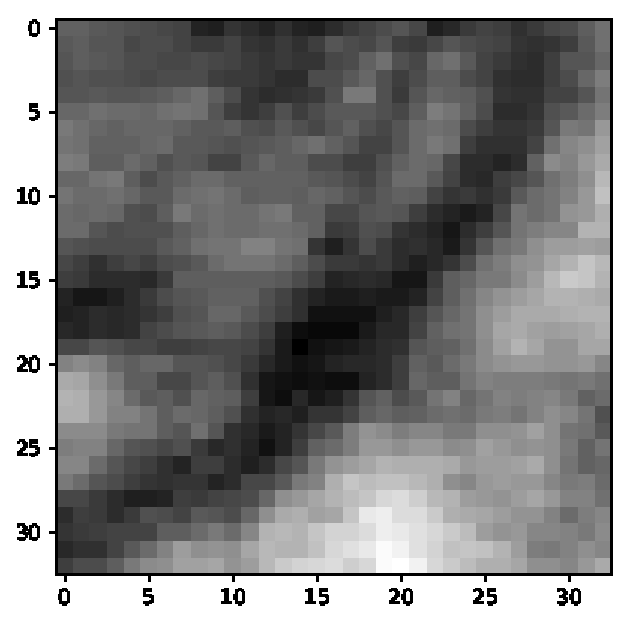
\includegraphics[width=\textwidth]{images/positive3.eps}
		\caption{}
	\end{subfigure}\\
	\vspace{0.25cm}
	\centering
	\begin{subfigure}[]{0.22\textwidth}
		\centering
		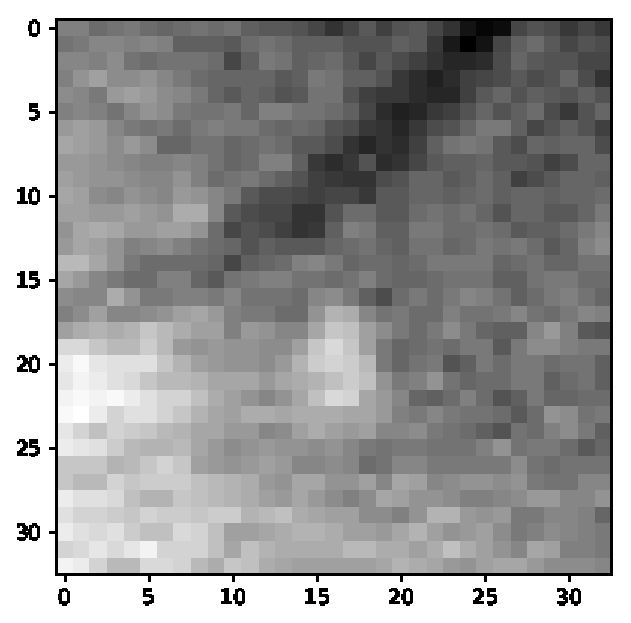
\includegraphics[width=\textwidth]{images/negative1.eps}
		\caption{}
	\end{subfigure}
	\hspace{1.55cm}
	\centering
	\begin{subfigure}[]{0.22\textwidth}
		\centering
		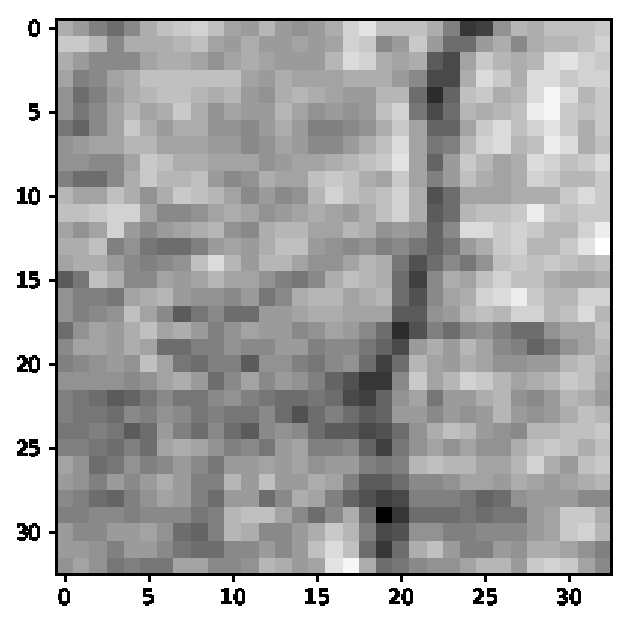
\includegraphics[width=\textwidth]{images/negative2.eps}
		\caption{}
	\end{subfigure}
	\hspace{1.55cm}
	\centering
	\begin{subfigure}[]{0.22\textwidth}
		\centering
		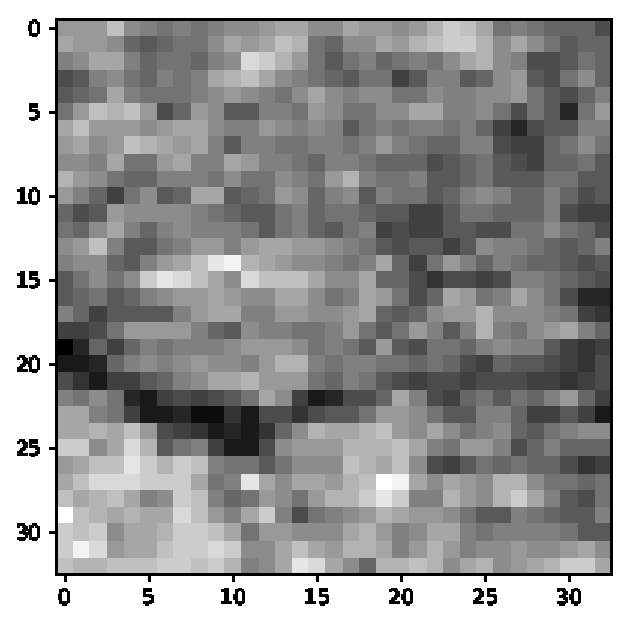
\includegraphics[width=\textwidth]{images/negative3.eps}
		\caption{}
	\end{subfigure}\\
	\caption{Examples of patches corresponding to pixels that are labeled as blood vessels (a)-(c) and patches corresponding to pixels that are labeled as background (d)-(f). The pixel that the label is related to is located at the center of patch.}
	\label{fig:example_patches}
\end{figure*}
\subsection{Developed Convolutional Neural Network}
\label{sec:computational_methods_developed_network}
The image is processed pixel by by and for each pixel a patch of size 33x33, cenetered at the pixel, is taken from the image and used in classification.
The developed convolutional neural network resembles that of Ref. \cite{tan}. However, instead of using three different patch resolutions in classification for a given pixel, only one resolution corresponding to 33x33 pixels from green channel is used in this work. The architecture of the developed neural network is shown in figure \ref{fig:net}. 
The input of size 33x33 pixels is fed to two convolutional layers with kernels of sizes 5x5. Each convolutional layer is followed by linear rectifying unit (RELU), a patch normalization layer and a max-pool layer with stride 2. The output of second max-pool layer is flattened and fed to fully connected layer followed by RELU. The RELU is followed by dropout layer with dropout probability of 0.5. Finally the output of the dropout layer is forwarded to last fully connected layer with single output. The output of the network is converted to probability using sigmoid function and the final class label is obtained using round operator.
\begin{figure*}[]
	\centering
	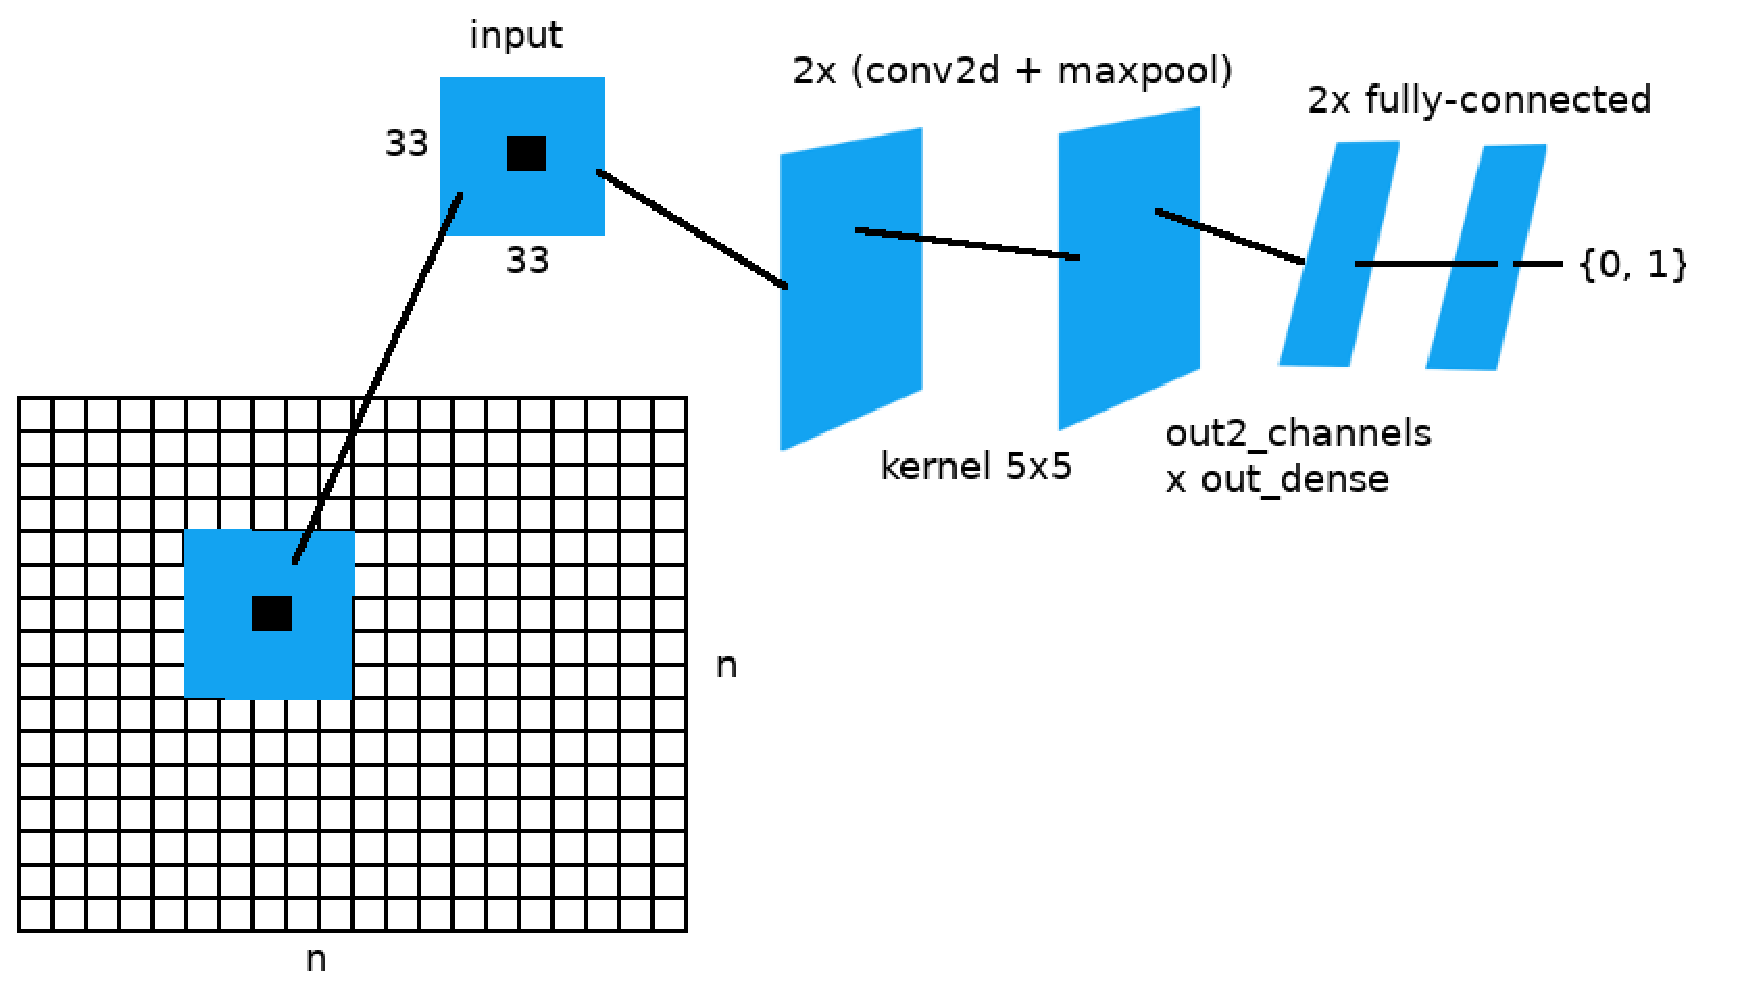
\includegraphics[width=0.7\textwidth]{images/net_cropped.eps}
	\caption{Architecture of the developed convolutional neural network.}
	\label{fig:net}
\end{figure*}

\subsection{Neural Network Training}
\label{sec:computational_methods_training_neural_network}
The developed method above contains three hyper parameters, the number of kernels in first and second convolution layer and the number of layers in first fully connected layer. Rest of the parameters, \textit{i.e.}, the kernel size and patch size were kept fixed. The optimal hyper parameters were found using random search. Ten different configurations were randomly sampled from given intervals that were $\lbrack$10, 35$\rbrack$, $\lbrack$10, 35$\rbrack$ and $\lbrack$200, 1200$\rbrack$ respectively for the hyper parameters. For each configuration the network was trained over 125 epochs using the train data set. In addition an early stopping criterion with tolerance of 0.01 and patience of 2 was used to avoid over fitting of the model. At the end of each epoch the validation loss, evaluated against the validation data set, was evaluated and used as input for early stopping criterion.

Stochastic gradient descent with patch size of 1000 and Adam optimizer\cite{adam}, initialized with learning rate of 1e-6 was used to optimize the network parameters. The final accuracy of the network, with given hyper parameters, was then obtained evaluating the accuracy against the test set. Final network, used in inference, was then constructed using the hyper parameters corresponding to best accuracy obtained. The final network was then retrained over 250 epochs or until early stop to get full convergence.

\subsection{Random forest classifier training}
\label{sec:computational_methods_training_random_forest}
The random forest classifier, that was used as a reference method, was implemented and trained using the Scikit-learn machine learning Python library. In used random forest classifier 200 estimators were used. The classifier was trained using the whole training data set.

\subsection{Inference}
\label{sec:computational_methods_inference}

\section{Results}
\label{sec:results}
\subsection{Optimal hyper parameters and the training accuracy for developed neural network}
\label{sec:results_training}
The results for the hyper parameter search, explained in section \ref{sec:computational_methods_training_neural_network}, are shown in Table \ref{tab:hyperparameter_searach_accuracies}. According to Table \ref{tab:hyperparameter_searach_accuracies} the best accuracy was obtained when the hyper parameters were set to 33x67x355. The final accuracy with these parameters for test set, after training over 250 epochs was 84.8\%.
\begin{center}
	\begin{table}[h]
		\begin{tabular*}{0.45\textwidth}{lclc}
			Configuration & Accuracy (\%) & Configuration & Accuracy (\%)\\
			\hline
			33x67x355 & 83.8 & 16x50x981 & 82.9\\
			29x42x709 & 83.7 & 18x63x1048 & 82.9\\
			29x49x871 & 83.5 & 27x58x359 & 82.4\\
			19x57x1158 & 83.3 & 10x64x1176 & 81.3\\
			20x60x256 & 83.2 & 14x49x638 & 80.1\\
		\end{tabular*}
		\caption{Results of the random hyper parameter search. The numbers in the configuration column indicates the number of kernels in the first and second convolution layers and the number of neurons in the first fully connected layer respectively. The accuracy is obtained running the trained network with the given hyper parameters against the test data set.}
		\label{tab:hyperparameter_searach_accuracies}
	\end{table}
\end{center}

\subsection{Training accuracy of the random forest classifier}
\label{sec:results_random_forest_training}
The obtained accuracy for the test data set using the trained random-forest classifier was around 88\%. Thus the obtained accuracy for the random-forest classifier is somewhat better than for the developed neural network.

\subsection{Inference}
\label{sec:results_inference}

\section{Conclusions}
\label{sec:conclusions}


\bibliography{references}

\appendix
\onecolumngrid
\section{Source Code}
\label{appendix:a}
\lstset{language=Python}
\subsection{Convolutional Network})
\begin{lstlisting}
import torch.nn as nn
import torch.nn.functional as F


class ConvNet(nn.Module):
def __init__(self, in_channels, out_channels1, out_channels2, out_dens):
super(ConvNet, self).__init__()
self.out_channels2 = out_channels2
self.conv1 = nn.Conv2d(in_channels, out_channels1, kernel_size=5, stride=1, padding=0)
self.batchn1 = nn.BatchNorm2d(out_channels1)
self.pool1 = nn.MaxPool2d(kernel_size=2, stride=2, padding=0)
self.conv2 = nn.Conv2d(out_channels1, out_channels2, kernel_size=5, stride=1, padding=0)
self.batchn2 = nn.BatchNorm2d(out_channels2)
self.pool2 = nn.MaxPool2d(kernel_size=2, stride=2, padding=0)

self.fc1 = nn.Linear(out_channels2 * 5 * 5, out_dens)
self.drop1 = nn.Dropout()
self.fc2 = nn.Linear(out_dens, 1)
self.sigmoid = nn.Sigmoid()

def forward(self, x):
x = F.relu(self.conv1(x))
x = self.batchn1(x)
x = self.pool1(x)
x = F.relu(self.conv2(x))
x = self.batchn2(x)
x = self.pool2(x)
x = x.view(-1, self.out_channels2 * 5 * 5)
x = F.relu(self.fc1(x))
x = self.drop1(x)
x = self.fc2(x)
return self.sigmoid(x)
\end{lstlisting}
\subsection{Training}
\begin{lstlisting}
from os.path import join
import time
import numpy as np
import torch
import torch.nn as nn
import torch.optim as optim
import sys
import argparse

from conv_models.convnet import ConvNet
from utils.loading import load_samples
from utils.regularization import EarlyStopping
from utils.loss_utils import compute_loss, compute_accuracy
from utils.parameter_search import random_search


def train(num_epochs, learning_rate, model_params, batch_size, x_train,
          y_train, x_valid, y_valid, x_test, y_test,
          device='cpu', save_model=False):

	net = ConvNet(1, model_params[0], model_params[1], model_params[2])
	net.to(device)

	criterion = nn.BCELoss()

	optimizer = optim.Adam(net.parameters(), lr=learning_rate)
	train_losses = []
	val_errors = []
	val_losses = []

	early_stop = EarlyStopping(tolerance=0.01, patience=2)

	for epoch in range(num_epochs):
		start_time = time.time()
		epoch_loss = 0
		for k in range(int(y_train.size / batch_size) - 1):
			start_ind = k * batch_size
			end_ind = (k + 1) * batch_size if (k + 1) * batch_size <
					   y_train.size else y_train.size
			x = torch.tensor(x_train[start_ind:end_ind, :], device=device,
				             dtype=torch.float)
			y = torch.tensor(y_train[start_ind:end_ind, :], device=device,
						     dtype=torch.float)

			# zero the parameter gradients
			optimizer.zero_grad()

			# forward + backward + optimize
			outputs = net(x)
			loss = criterion(outputs, y)
			epoch_loss += np.asscalar(loss.cpu().data.numpy())

			loss.backward()
			optimizer.step()

		# Print accuracy after every epoch
		train_losses.append(epoch_loss)
		validation_accuracy = compute_accuracy(net, x_valid, y_valid)
		val_errors.append(validation_accuracy)
		validation_loss = compute_loss(net, x_valid, y_valid)
		val_losses.append(validation_loss)
		time_taken = (time.time() - start_time)
		print('Accuracy of the network on epoch %d %%' % epoch + ': %f %%' %
		      (100 * validation_accuracy) +
		'validation loss: %f ' % validation_loss + 'train loss: %f ' %
		 epoch_loss + ' took %f' %time_taken + 'seconds')
	
		if early_stop.stop_criterion(val_losses):
			print('Stop after %d epochs' % epoch)
			break

	test_accuracy = compute_accuracy(net, x_test, y_test)
	if save_model:
	save_filename = join('saved_models',
	'convnet_' + str(model_params[0]) + 'x' + str(model_params[1]) + 'x' +
	str(model_params[2]) + '.pth')
	torch.save(net.state_dict(), save_filename)
	np.savez(join('saved_models', 'training_losses.npz'),
	train_losses=train_losses,
	val_losses=val_losses,
	final_accuracy=test_accuracy)

	print('Final test accuracy: %f %%' % (100 * test_accuracy))
	return test_accuracy


def optimize_hyper_parameters(num_epochs, learning_rate,
                              num_combinations, batch_size,
                              x_train, y_train, x_valid,
                              y_valid, x_test, y_test):

range1 = [10, 35]
range2 = [35, 70]
range3 = [200, 1200]

parameter_combinations = random_search(num_combinations, range1, range2, range3)
hyper_parameters = []
accuracies = []

for n1, n2, n3 in parameter_combinations:
accuracy = train(num_epochs, learning_rate, [n1, n2, n3], batch_size, x_train,
			     y_train, x_valid, y_valid,
			     x_test, y_test)
hyper_parameters.append([n1, n2, n3])
accuracies.append(accuracy)
print('accuracy with parameters [' + str(n1) + ', ' + str(n2) + ', ' + str(n3) + ']
	 ' + str(accuracy))

hyper_parameters = np.array(hyper_parameters)
accuracies = np.array(accuracies)
np.savez(join('saved_models', 'hyperparameters4.npz'),
hyperparameters=hyper_parameters,
accuracies=accuracies)

ix = accuracies.argsort()[-1::-1]

print(accuracies[ix])
print(hyper_parameters[ix, :])


def train_random_forets_classifier(x_train, y_train, x_test, y_test, save_model=False):

from sklearn.ensemble import RandomForestClassifier
from sklearn.metrics import accuracy_score
import pickle

x_train = np.reshape(x_train, (x_train.shape[0], x_train.shape[2] * x_train.shape[3]))
x_test = np.reshape(x_test, (x_test.shape[0], x_test.shape[2] * x_test.shape[3]))
y_train = np.reshape(y_train, (y_train.size, ))
y_test = np.reshape(y_test, (y_test.size, ))
classifier = RandomForestClassifier(n_estimators=200, verbose=1, n_jobs=-1)
classifier.fit(x_train, y_train)
pred_test = classifier.predict(x_test)
rf_accuracy = accuracy_score(y_test, pred_test)
print("Accuracy of random forest: {:.2f}".format(rf_accuracy))

if save_model:
pickle.dump(classifier, open('saved_models/random_forest.p', 'wb'))

classifier = pickle.load(open('saved_models/random_forest.p', 'rb'))
pred_test = classifier.predict(x_test)
rf_accuracy = accuracy_score(y_test, pred_test)
print("Accuracy of random forest: {:.2f}".format(rf_accuracy))


def main(args):

parser = argparse.ArgumentParser()
parser.add_argument('--num_epochs', default=1, type=int)
parser.add_argument('--batch_size', default=1000, type=int)
parser.add_argument('--learning_rate', default=1e-6, type=float)
parser.add_argument('--optimize_hyperparameters', default=False, type=bool)
parser.add_argument('--save_model', default=False, type=bool)
parser.add_argument('--num_combinations', default=10, type=int)
parser.add_argument('--use_random_forest', default=False, type=bool)
args = parser.parse_args(args)

use_random_forest = args.use_random_forest
num_epochs = args.num_epochs
batch_size = args.batch_size
learning_rate = args.learning_rate
hyper_parameter_optimization = False#args.optimize_hyperparameters
num_combinations = args.num_combinations
save_model = args.save_model

(x_train, y_train), (x_valid, y_valid), (x_test, y_test) = load_samples(2000)

if use_random_forest:
train_random_forets_classifier(x_train, y_train, x_test, y_test, save_model)
elif hyper_parameter_optimization:
optimize_hyper_parameters(num_epochs, learning_rate, num_combinations, batch_size,
x_train, y_train, x_valid, y_valid, x_test, y_test)
else:
train(num_epochs, learning_rate, [33, 67, 355], batch_size, x_train, y_train, x_valid,
y_valid, x_test, y_test, device='cpu', save_model=save_model)


if __name__ == '__main__':
main(sys.argv[1:])
\end{lstlisting}

\end{document} 






